\documentclass[conference,11pt]{IEEEtran}
\usepackage[utf8]{inputenc}
\usepackage[english]{babel}
\usepackage[left=1in,right=1in,top=1in,bottom=1in,footskip=.25in]{geometry}
\usepackage{cite}
\usepackage{hyperref}
\usepackage{fancyhdr}
\usepackage{datetime}
\usepackage{amsmath}
\usepackage{url}
\usepackage{subfig}
\usepackage{float}
\usepackage{graphicx}
\graphicspath{ {images/} }
\usepackage{setspace}
%\setlength{\parskip}{1em}
\pagenumbering{arabic}
\pagestyle{fancy}

\usepackage[numbered,framed]{matlab-prettifier}
\usepackage[T1]{fontenc}
\usepackage[scaled]{beramono}
\lstset{
  style              = Matlab-editor,
  basicstyle         = \mlttfamily,
  escapechar         = ",
  mlshowsectionrules = true,
}

\title{Feature Transfer Learning for Automated Lung Cancer Detection}
\author{
    \IEEEauthorblockN{Benjamin Hillmann}
    \IEEEauthorblockA{
        \today
    }
}

\begin{document}
\onecolumn
\maketitle

\begin{abstract}
In order to assess early risk factors of high-risk patients for lung cancer, a non-invasive low-resolution computed tomography (CT) scan is administered. The results of the CT scan are a 3D intensity image of the patients chest region. The important features of this scan are pulmonary nodules or small masses within the lungs, that can be classified as either benign (non-cancerous) or malignant (cancerous). Typically, a radiologist will analyze the scans to determine the diagnosis of the nodules and the patient. With advances in technology, experiments are being conducted with computer-aided diagnosis (CAD) technologies to synergize with human expertise analysis and reduce false positive diagnosis. In this work, abstract image features from deep neural networks are extracted from each slice of the CT scan. These abstract features are then combined and their correlation and prediction capabilities for malignancy are assessed.
\end{abstract}

\section{Introduction}

Cancer is one of the leading causes of death worldwide, accounting for 8.8 million deaths in the year 2015 \cite{noauthor_who_nodate}. Within the United States, lung cancer is the deadliest form as shown in \textit{Figure~\ref{fig:cancer}} and costs billions in dollars in health care costs \cite{noauthor_united_nodate}. With current medicine technologies, many of the current cases of lung cancer can be prevented. Techniques to prevent the development of cancer include avoiding risk factors, raising awareness of prevention strategies, and early stage detection and management of cancer patients.

%%% fig:cancer
\begin{figure}[hbt]
    \centering
    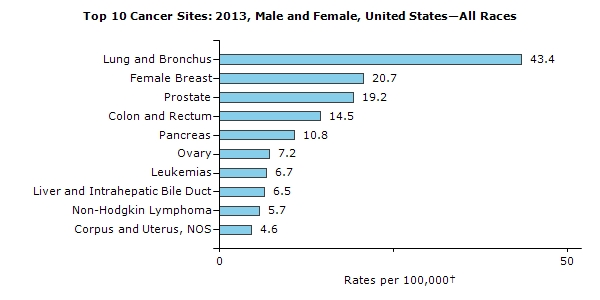
\includegraphics[width=0.8\linewidth]{figures/plot_top_ten_cancers.jpg}
    \caption{Death rates of the most common forms of cancer in the United States per 100,000 people. Lung and bronchus cancer has the highest mortality rate, with more than twice the mortality rate of the second deadliest form of cancer.}
      \label{fig:cancer}
\end{figure}

The mortality rate of cancer can be reduced through early detection and diagnosis. A common early stage detection technique is to administer a low-resolution computed tomography (CT) scan. A benefit of a CT scan is that they are non-invasive which make them low-risk to administer. The results of a CT scan are a 3D intensity image of the patients chest region. The important features within a scan are nodules or masses within the lungs, that can be classified as either benign (non-cancerous) or malignant (cancerous). Typically, a radiologist will analyze the scans to determine the diagnosis of the nodules and the patient. With advances in technology, experiments are being conducted with computer-aided diagnosis (CAD) technologies to aid with human expertise analysis and reduce false positive diagnosis.

The purpose of this analysis is to develop a CAD procedure to classify the risk of a patient that underwent a CT for having or developing cancer within the next year. The input for the CAD is simply the 3D intensity scans of the upper chest region of patients with a predetermined high-risk of having cancer. The output of the classifier is the risk that the patient will develop lung cancer within the next year. The state of the art algorithms in computer vision and machine learning described in this analysis reduces the number of false positive diagnosis made by current CAD technology \cite{sun_automatic_2017, ronneberger_u-net:_2015}. The successfulness of this approach will allow patients to receive quicker access to life-saving intervention, and give radiologists more time to provide that intervention.

The approach outlined in this paper is an experiment in the transferability of abstract features learned within the inner layers of a deep neural network. An original deep neural network was trained on the semantic tags given to the natural image database Imagenet \cite{russakovsky_imagenet_2015,yosinski_how_2014,he_deep_2015}. The classification layers are removed from the original network, and the weights output from the remaining layers are treated as the input feature space. The abstract features are averaged across all layers in the image, and the resulting embedding is input to a gradient boosting machine. Analysis of the method shows that the proposed methods outperforms a random and majority class classifier. Furthermore, the specific feature space outperforms a boosting gradient machine on a random feature space. This approach shows the effectiveness of the generalization of feature embeddings provided by deep neural networks trained in non-related domains to targeted problems. This approach is generally useful when the number of samples to train is relatively low due to complexities or cost of dataset collection, such as with biomedical datasets.

\section{Background}

The goal for this project was to apply techniques in ongoing machine learning and artificial intelligence research to accurately predict the risk for a patient to develop lung cancer. This project was an entry into the Data Science Bowl, an annual competition hosted by the data science competition website  \href{https://www.kaggle.com/c/data-science-bowl-2017}{Kaggle}. This competitions aligns with the Cancer Moonshot initiative, that has the goal of utilizing intelligent data analysis to advance screening, care and prevention of cancer. The final goal of the initiative is to end cancer entirely.

\subsection{Dataset}
The data for this project is being hosted by the data science competition website \href{https://www.kaggle.com/c/data-science-bowl-2017}{Kaggle} as a part of the 2017 Science Bowl. The data includes over a thousand low-dose CT images from patients that are high-risk for lung cancer. The format they are provided in is DICOM, and contains 3D segmented intensity scans of various resolutions. An example slice from one of the 3D images is shown in \textit{Figure~\ref{fig:slice}}.

%%% slice
\begin{figure}[htb]
    \centering
         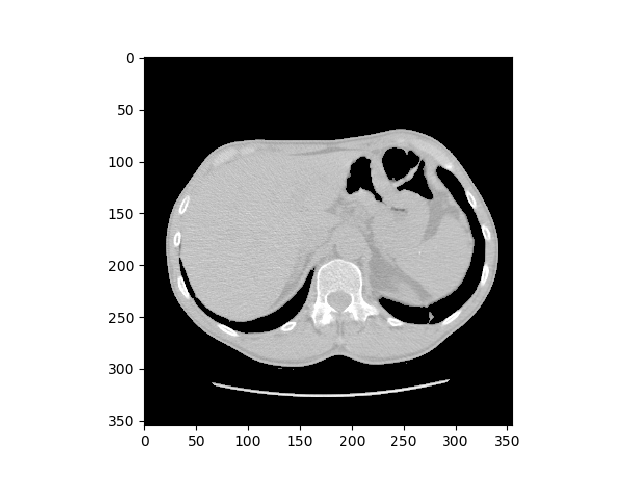
\includegraphics[width=0.8\linewidth]{figures/plot_slice.png}
	\caption{An example slice from a CT image. The intensity values are projected into a grayscale color map.}
    \label{fig:slice}
\end{figure}

The competition was formatted in two stages. The first stage, labeled as stage1, was designed to build and test models. The data for stage1 was separated into a training, meaning labeled with being cancerous or not, and a test set, which contains no labels. A competitor has access to download all the data for stage1, build a supervised machine learning regression on the training set, then upload their predictions for the stage1 test set to the website leaderboard. The input for the computational pipeline was the DICOM images, and the output target was the risk $y$ in the range $y \in (0,1)$ that a patient develops lung cancer in the next year. The leaderboard was ordered by submissions with the lowest logloss on the training set. The logloss of the test set is defined below:

%%% LogLoss
$$ \textrm{logloss} = - \frac{1}{n} \sum_{i=1}^n \left[ y_i \log(\hat{y}_i) + (1 - y_i) \log(1 - \hat{y}_i)\right]. $$

The second stage of the competition, labeled as stage2, contained no labeled training data. The purpose of stage2 was to reduce over-training on the dataset, eliminate leaderboard hacking of various submission for better scores, and to evaluate the bias in each of the submissions. There is a public and a private leaderboard in stage2. The public leaderboard was a small and unknown subsample of the stage2 test data. The private leaderboard contained the rest of the testing data not included in the public leaderboard and was used for the final evaluation of the submissions based on logloss. The sample size and disk usage for each of the stages are shown in \textit{Figure~\ref{fig:dataset}}.

%%% dataset
\begin{figure}[htb]
    \centering
    \[
      \begin{array} {|c|c|c|c|c|}
        \hline
        & \textnormal{Train Set} & \textnormal{Test Set} & \textnormal{Size (GB)} & \textnormal{Size Compressed (GB)} \\ \hline
        \textnormal{stage1}  & 1398 & 199 & 139 & 112 \\ \hline
        \textnormal{stage2}  & 0 & 507 & 91.1 & 69.5\\ \hline
      \end{array}
    \]
    \caption{Summary statistics for the number of samples and disk used for the competition dataset. The stage1 of the competition was used for evaluation and submission of the models. The stage2 was for final evaluation of the competition to show the generalization of the models, to guard against information leakage, leaderboard hacking, and over-training. File compression was enabled on the hard drive to reduce space and show the redundancy in the data.}
    \label{fig:dataset}
\end{figure}

\subsection{Deep Neural Networks for Image Classification}

Deep neural networks have been utilized for breakthrough results in image classification \cite{he_deep_2015}. For example, consider the problem of semantic tagging and the Imagenet 2012 dataset \cite{russakovsky_imagenet_2015}. Semantic tagging is the process of annotating an image with keywords that appeared in that image. In the ImageNet 2012 dataset,  there are 1.28 million training images with human annotated 1,000 classes or semantic tags. A single image may contain any number of semantic tags. There are 50,000 validation images, with the objective of automatically tagging these images with as little error as possible. An example image and classification using a deep neural network is shown in \textit{Figure~\ref{fig:elephant}}.  The architecture of deep neural networks allows the combination of low, mid and high level image features that are enriched by many stacked layers. These neural networks have been shown, when properly tuned, to provide the best end-to-end solution with the lowest error for semantic tagging on the ImageNet dataset. 

%%% elephant
\begin{figure}[htb]
  \centering
  \begin{minipage}[c]{0.38\textwidth}
    \centering
    \begin{tabular} {|c|c|}
            \hline
            \textnormal{Semantic Tag} & \textnormal{Similarity} \\ \hline
           African elephant & .473 \\ \hline
           Indian elephant & .250 \\ \hline
           tusker & .016 \\ \hline
           dugong & .016\\ \hline
           ram & .015 \\ \hline
          \end{tabular}
  \end{minipage}
  \begin{minipage}[c]{0.58\textwidth}
    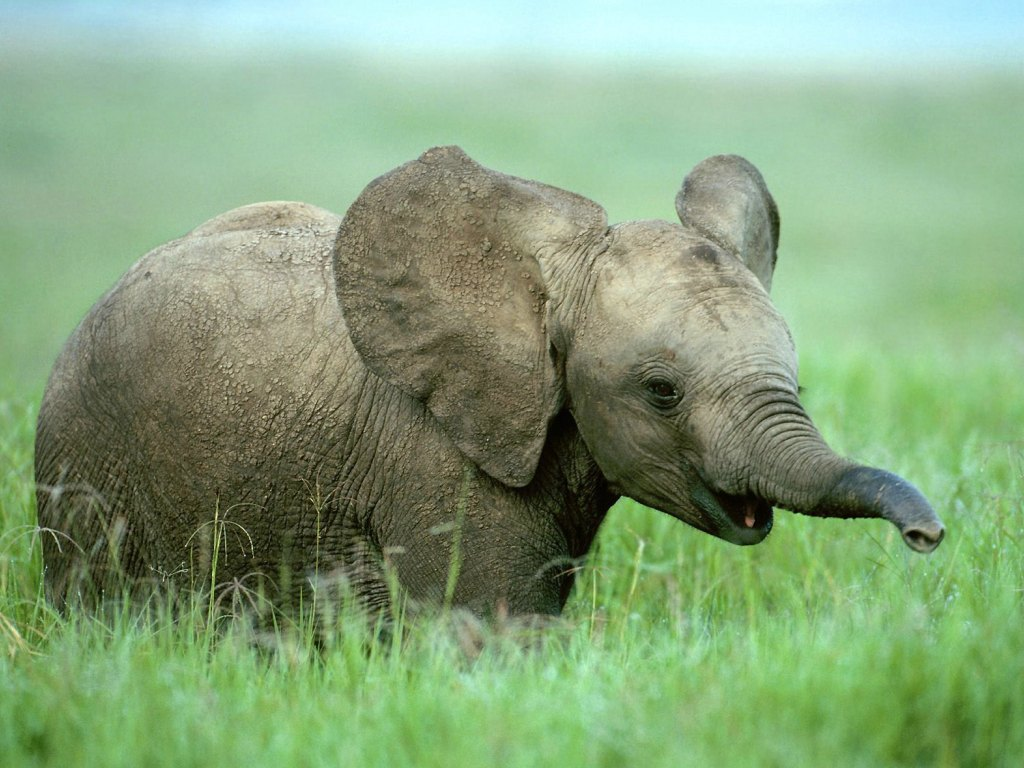
\includegraphics[width=\textwidth]{figures/plot_elephant.jpg}
  \end{minipage}
  \caption{An example image and annotation from a neural network trained on the ImageNet 2012 dataset. On the left, is the semantic tags and the confidence the neural network has in them. On the right, is the example image to be annotated.}
  \label{fig:elephant}
\end{figure}

\subsection{Nodule Segmentation}

Previous work for risk regression using CAD has been focused around image segmentation. In the case of lung cancer, the 3D images are segmented into voxels that contain nodules. Nodules are small masses within the lung, and their properties, such as shape and size, are what human annotators use for diagnosing cancer risk. For this task, a specific architecture of a convolution neural network (CNN) has been trained to detect nodules given an image \cite{ronneberger_u-net:_2015}. The training set size $N$ for this network architecture are assumed to be small, $10 < N < 10,000$. The training set utilized in this paper contained radiologist segmented images that are cut around nodules. The network is designed to maximize the trade-off between classifier localization and context accuracy. Localization is the ability of the classifier to correctly label each pixel of an image as containing a nodule or not. The contextual accuracy is the ability to predict each group of pixels accordingly as a nodule, that is, the number of nodules detected is correct. The network architecture describes meets these goals by a dual channel approach, with one channel being traditional convolution operations for contextual features, and the second channel being an up-sampling architecture for pixel localization.

After an image is segmented, properties of each individual voxel is regressed towards being malignant. Often times, after nodule segmentation of an image is complete, there exists many false positive candidate nodules. An approach to increase precision to utilize a graph cutting algorithm followed by a CNN architecture specifically designed to reduce false positives \cite{sun_automatic_2017}. After false positive reduction, the final candidate nodules are analyzed by a CNN to predict malignancy.

\subsection{Transfer Learning}

The first few layers of deep neural networks trained on natural images tend to lend themselves to the same phenomena, they learn color blobs and abstract edge filters \cite{yosinski_how_2014}. These features do not limit themselves to particular tasks or datasets and nevertheless are common between many of them. Therefore, when the sample size for a particular dataset is small, it is often the case that these first few layers of a previously learned dataset can be transferred successfully as the initialization weights for a new classification task. The transferability of these edge weights have been shown to rely on two issues. The first issue is the specialization of layers to their original task. The second issue is the optimization of co-adapted layers that were split from the original network. Even with these issues, often times the transferability of these weights lends itself to fast stabilization of new classification tasks. The transferability of features also decreases as the difference between the original task and the target task increases. However, even with vastly different original and target tasks, initialization with pre-trained weights is often better than initialization with random weights. Finally, initialization often times provides better classification error than a finely tuned network architecture for a new dataset.

\section{Methods}

In order to determine the risk of a patient developing lung cancer from a CT scan, the features to search for are pulmonary nodules \cite{armato_lung_2011}. A pulmonary nodule is a small mass in the lung that are of primary concern because they are often formed by cancer. Finding a pulmonary nodule in a CT scan is a difficult task due to the relative size of the nodules compared to the size of the image \cite{vansteenkiste_predicting_nodate}. Furthermore, a single malignant nodule determines the diagnosis for the entire scan.

For context, consider the  LUng Node Analysis (LUNA) Grand Challenge \cite{setio_validation_2016}. The average CT scan has a volume of approximately 400mm$^3$, while the average radius of a malignant nodule in the LUNA dataset is 4.8 mm. This means that in order to correctly classify a given CT scan, the classifier needs to find a mass that is ~500,000 times smaller than the input volume. Finding these small masses is what makes it so difficult for radiologists and CAD alike. If a malignant nodule is missed from a radiologist during the image segmentation, the diagnosis of the entire scan becomes incorrect.

The problem of the large search space with a small target feature becomes exacerbated in the Data Science Bowl challenge, because the patient scan may not even contain malignant nodules. This is because every patient in the LUNA dataset is already diagnosed with lung cancer. In the Data Science Bowl, the patients are sent for a screening CT scan where they might not have formed nodules yet. With only the labels given in the training set, it is probably impossible to have a machine learning classifier learn past the majority class bias in the dataset.

To address these challenges, I implemented formation of transfer learning.

\subsection{Data Normalization}

Due to the variances in human body sizes and users operating the CT machines, each of the CT scans were taken with various zoom factors. To account for these various resolutions, each of the images were standardized so that a voxel in the image represented 1m$^2$. The image zoom standardization was done with smoothing over a first order polynomial.

The standard unit of measurement in CT scans is the radio-density measurement the Hounsfield Unit (HU). Utilizing this standard unit allows us to easily threshold the dataset to specific substances in the body as shown in the scale in \textit{Figure~\ref{fig:hounsfieldunits}}. The images in the dataset, however, contain different scalings for radiodensity that is dependent on the machine taking the scan \cite{noauthor_data_nodate}. The images were normalized across machine dependent batches to account for this affect. Thresholding the new images at a specific radio-density for lung and bones is shown in \textit{Figure~\ref{fig:boneslungs}}. Some of the CT scanners have cylindrical scanning bounds but the output images are square, resulting in the images having extra empty pixels. These pixels are typically bounded by -2000, and they can reset to 0 as air as shown in \textit{Figure~\ref{fig:hist}}. Lastly, the total histograms are standardized between 0 and 1.
%%% hist
\begin{figure}[htb]
    \centering
      \subfloat[The distribution of the pixel intensity values before preprocessing. Notice the over representation of pixels that are at the value -2000.] {
         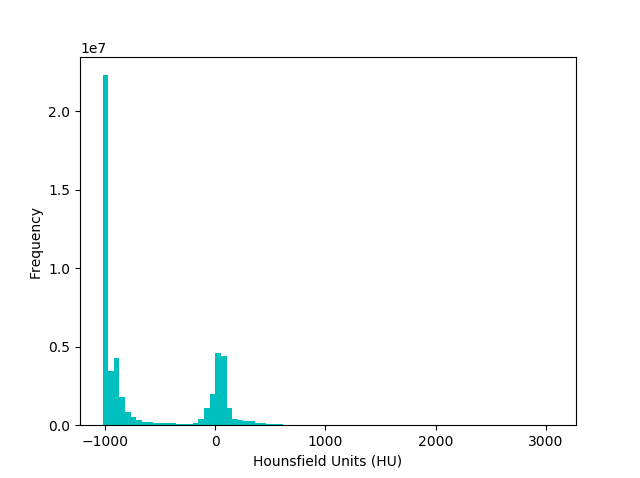
\includegraphics[width=0.4\linewidth]{figures/plot_hist_hu.png}
      }
    	\hspace{0.02\linewidth}
      \subfloat[The distribution of pixel intensity values after preprocessing. The bounds of the pixels $v$ were thresholded such that $v \in \lbrace 0,1 \rbrace$. Also notice the clipping of the values.] {
          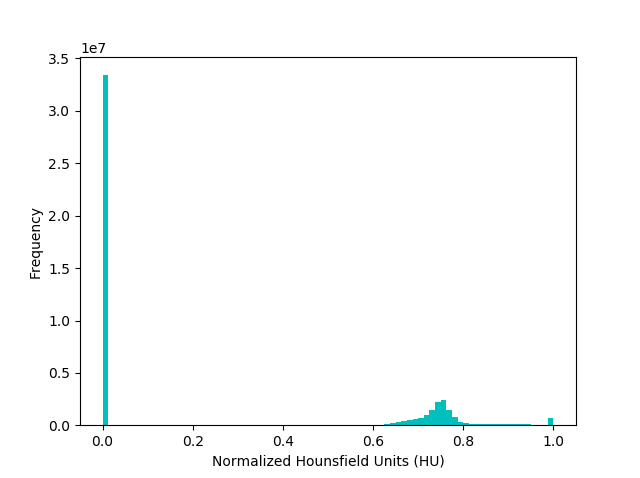
\includegraphics[width=0.4\linewidth]{figures/plot_hist_norm_hu.png}
          }
      \caption{Pixel intensity distributions before and after preprocessing.}
      \label{fig:hist}
\end{figure}

%%% hounsfieldunits
\begin{figure}[ht]
    \centering
	\begin{tabular} {|c|c|}
    	\hline
        \textnormal{Substance} & \textnormal{HU} \\ \hline
        \textnormal{Air} & -1000 \\ \hline
        \textnormal{Lung} & -500 \\ \hline
        \textnormal{Fat} & 0 \\ \hline
        \textnormal{Water} & +15 \\ \hline
        \textnormal{CSF} & +30 \\ \hline
        \textnormal{Kidney} & +30\\ \hline
        \textnormal{Blood} & +30 \\ \hline
        \textnormal{Muscle} & +10 \\ \hline
        \textnormal{Grey matter} & +37 \\ \hline
        \textnormal{White matter} & +20 \\ \hline
        \textnormal{Liver} & +40 \\ \hline
        \textnormal{Soft Tissue, Contrast} & +100 \\ \hline
        \textnormal{Bone} & +700 \\ \hline
    \end{tabular}
    \caption{Various HUs for different substances within the body \cite{noauthor_hounsfield_2017}.}
    \label{fig:hounsfieldunits}
\end{figure}

%%% boneslungs
\begin{figure}
    \centering
      \subfloat[Image thresholded for the HU of bones.] {
         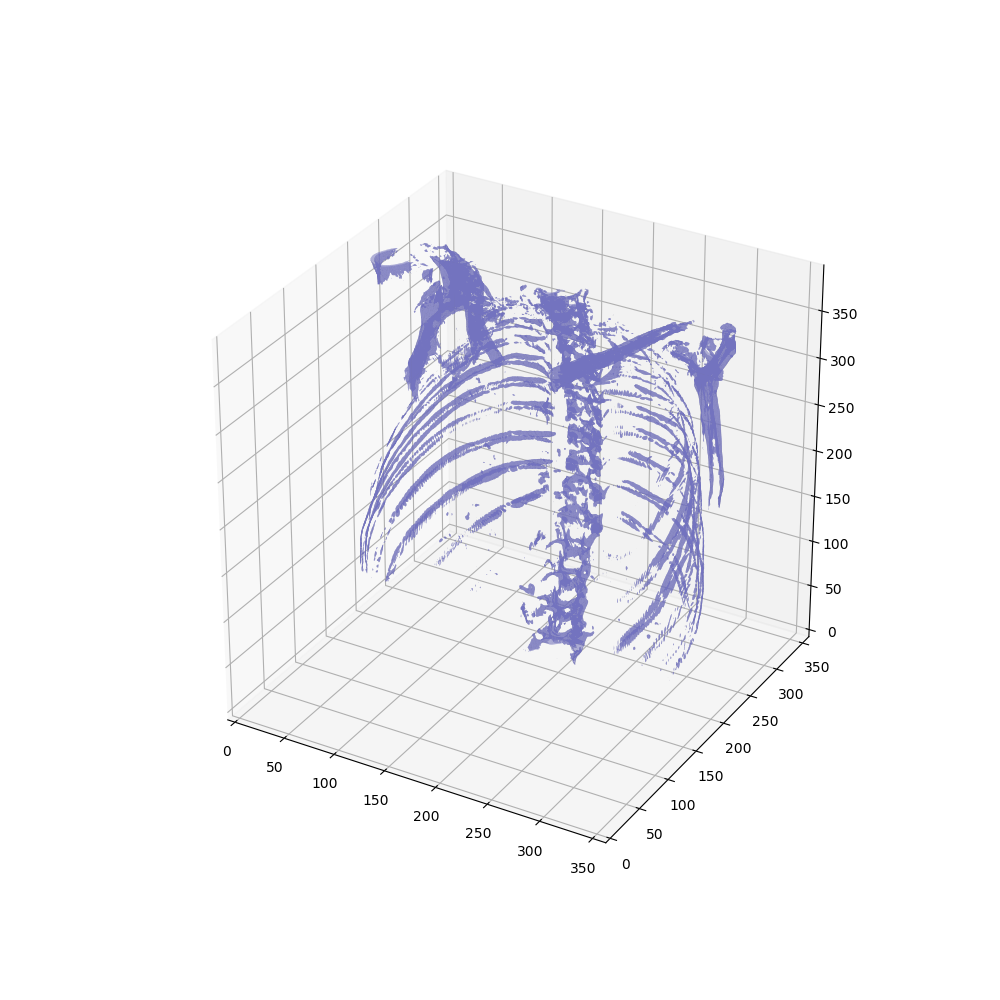
\includegraphics[width=0.4\linewidth]{figures/plot_bones.png}
      }
    	\hspace{0.02\linewidth}
      \subfloat[Image thresholded for the HU of lungs.]{
          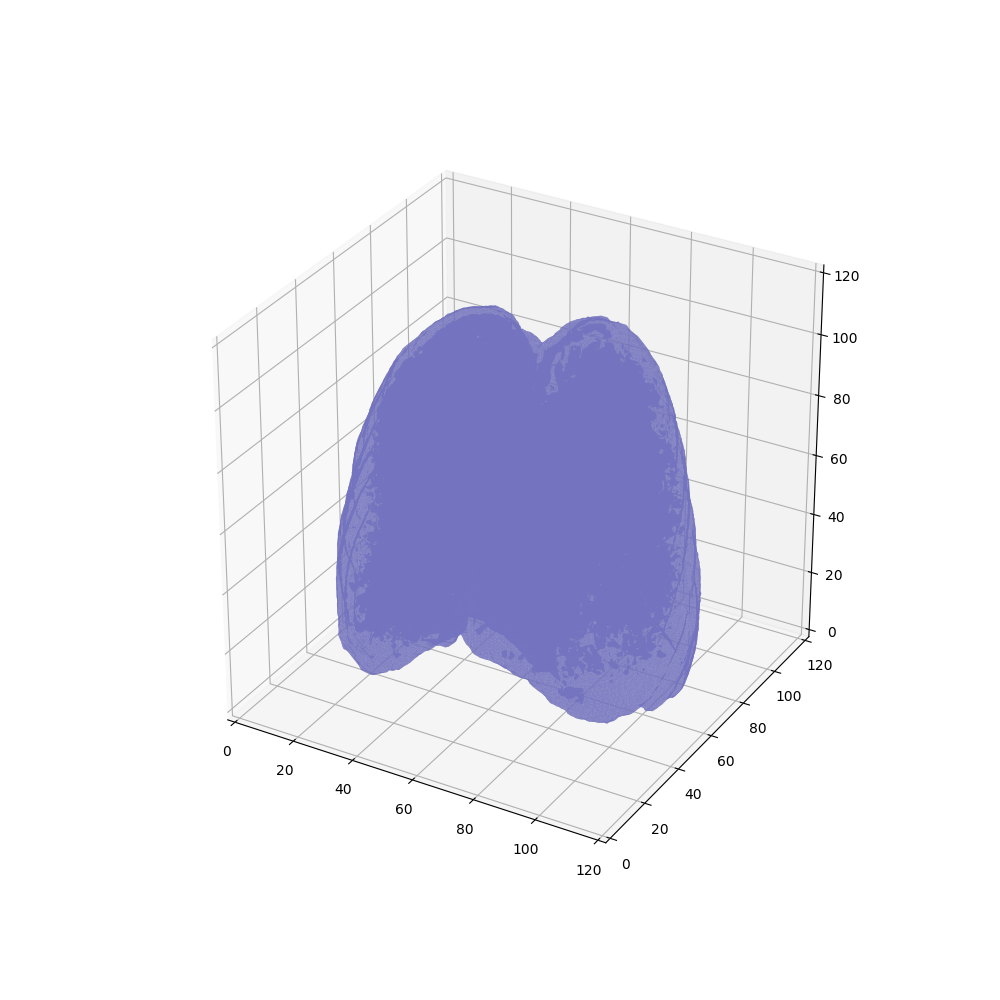
\includegraphics[width=0.4\linewidth]{figures/plot_lungs.png}
      }
      \caption{Resulting 3D reproductions of a scan thresholded for bones (a) and lungs (b).}
      \label{fig:boneslungs}
\end{figure}

The original images were various resolutions of single-channel (grayscale) 3D images. In order for them to work inside of the network architecture, they needed to be converted into the three-channel (RGB) channels. Each consecutive three slices were concatenated and stacked into their respective channel. An example of the resulting concatenated slices for a single scan are shown in \textit{Figure ~\ref{fig:slices}}.

%%% slices
\begin{figure}
    \centering
         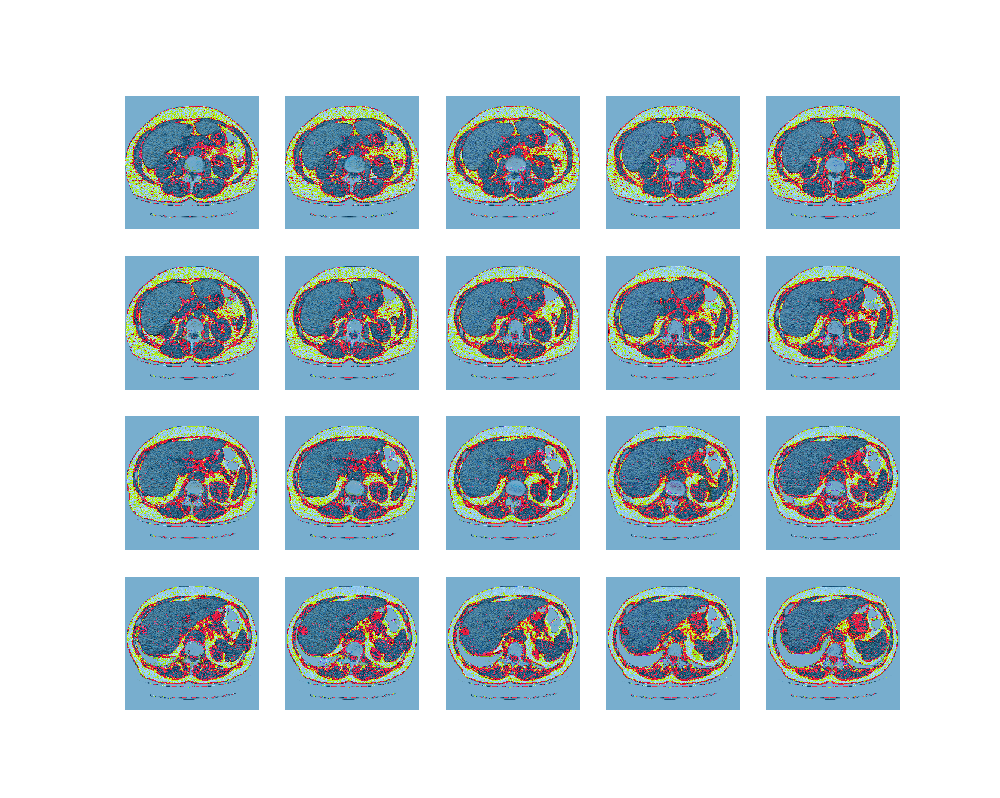
\includegraphics[width=0.8\linewidth]{figures/plot_slices.png}
      \caption{Example encoding of a single 3D scan into multiple RGB images.}
      \label{fig:slices}
\end{figure}

\subsection{Network Architecture}

Architecture for feature extraction was modeled as the ResNet50 architecture as shown in \textit{Figure~\ref{fig:slices}} \cite{he_deep_2015}. This specific architecture was designed for stabilizing the convergence of deep neural networks. It was shown that the more layers, also known as creating deeper neural networks, a neural network architecture is, the better it performs on computer vision tasks. Besides the convergence issues for these network, they also have shown to have a degradation problem where accuracy becomes saturated and then rapidly decreases in deeper layers. These issues were taken care of in the ResNets by building 'blocks' of stacked layers that learn off of the residuals of the previous blocks. This approach was shown to increase the stabilization and the performance of the deeper neural networks on various tasks.

%%% resnet50
\begin{figure}
    \centering
    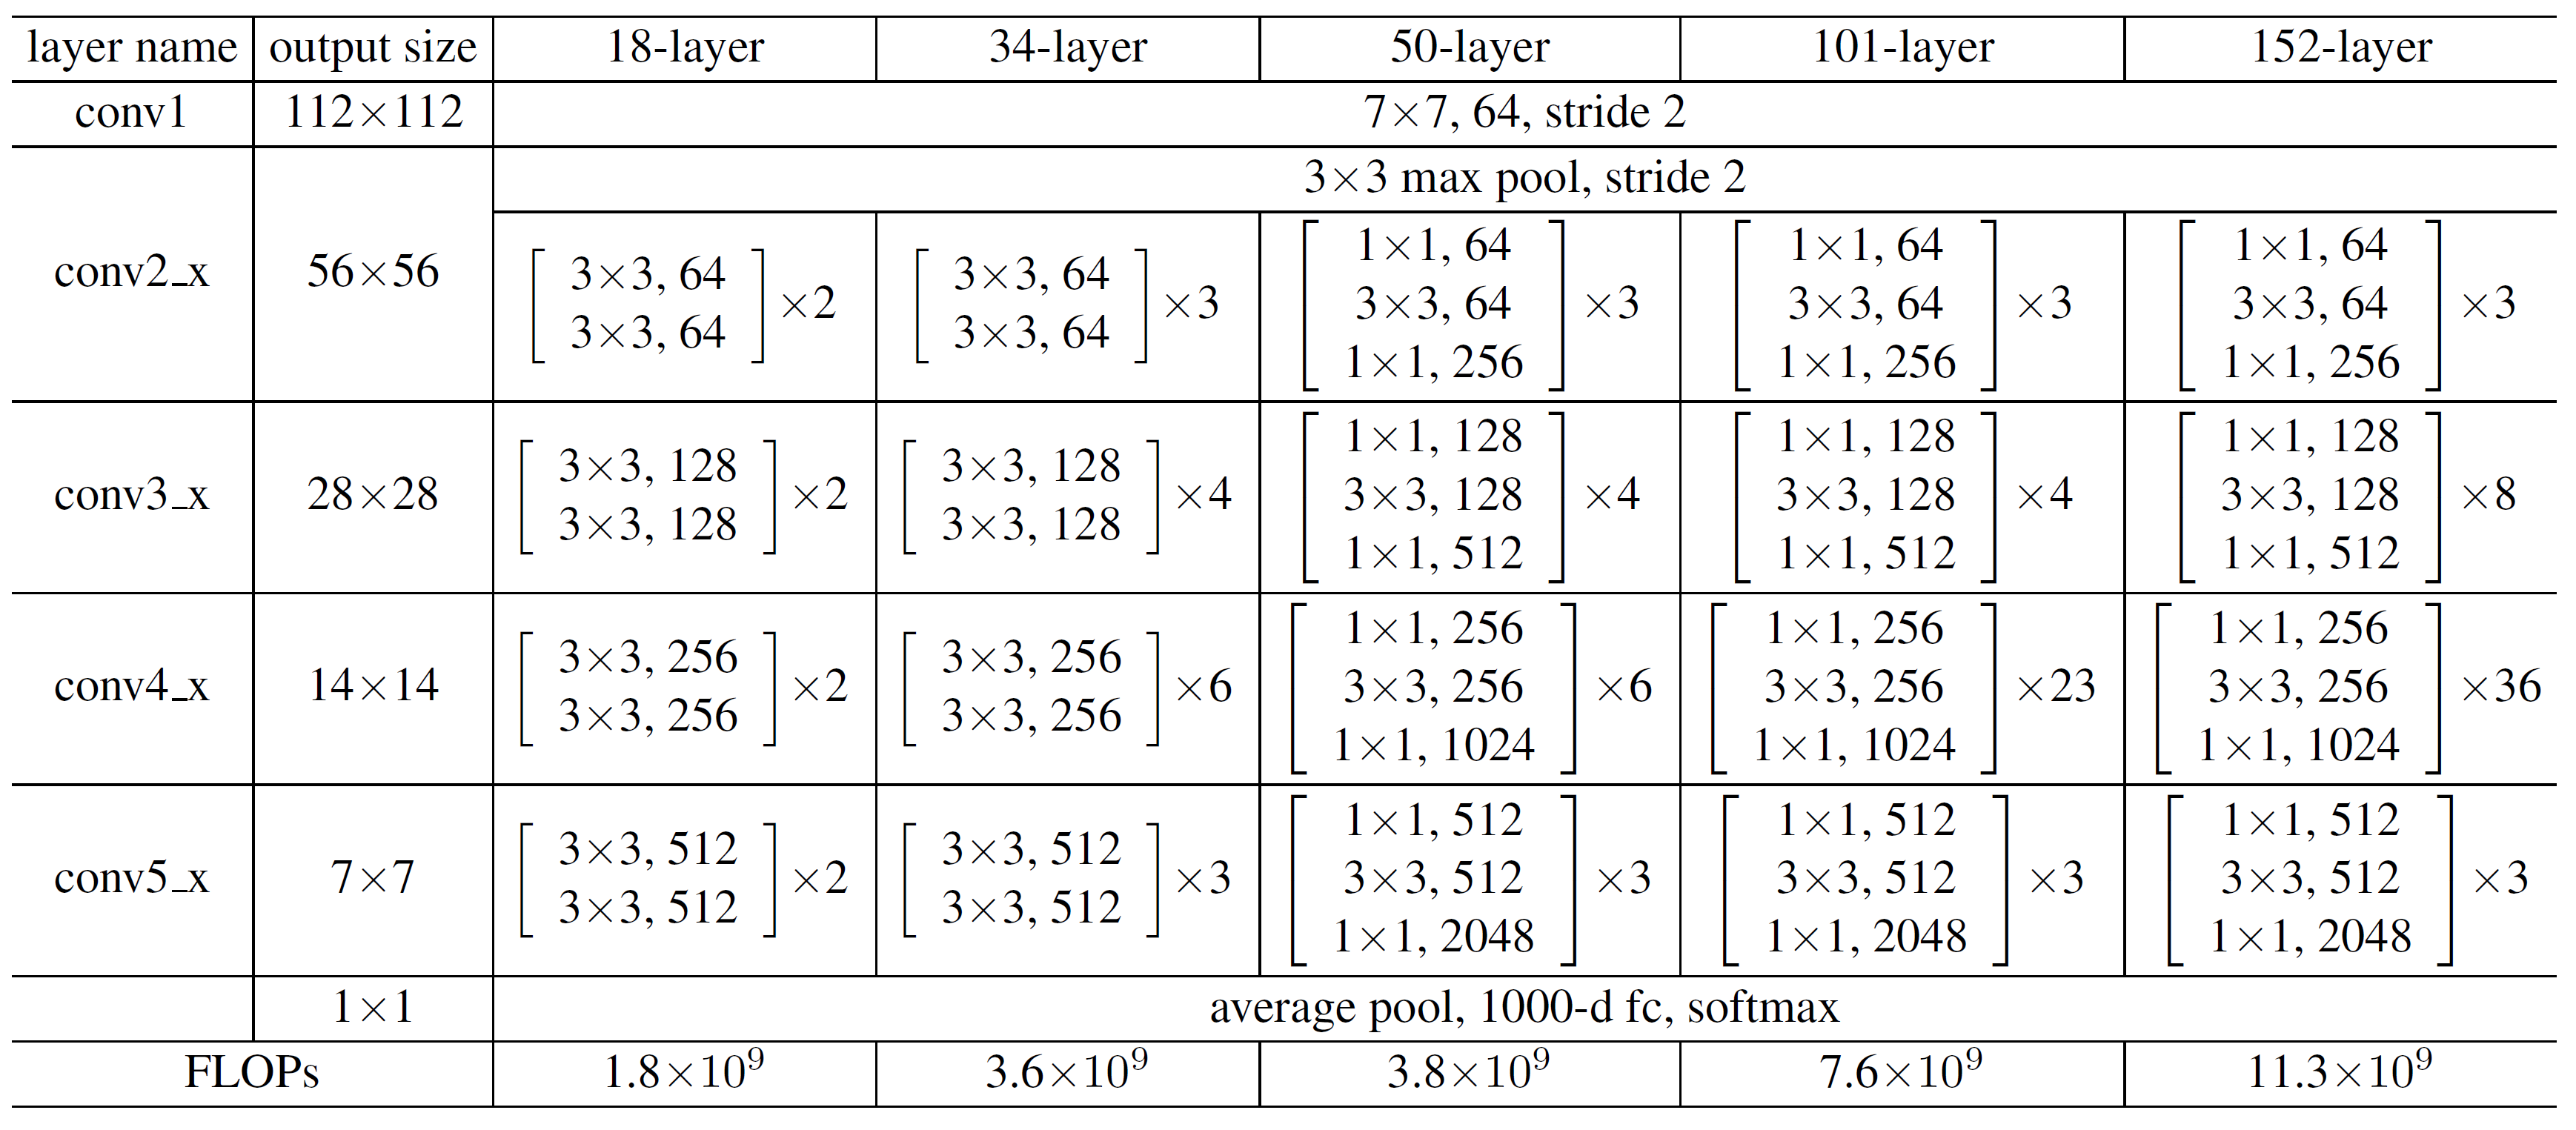
\includegraphics[width=0.8\linewidth]{figures/plot_resnet50.png}
    \caption{The architectures used for semantic tagging ImageNet from the original ResNet paper \cite{he_deep_2015}. The brackets indicate the number of layers inside that are stacked.}
    \label{fig:resnet50}
\end{figure}

The baseline network used with transfer learning was the exact weights of the ResNet50. However, the last prediction layer and labels were truncated so that the more abstract 'shape' features could be used. In this way, rather than saying there is a high probability that there is an 'elephant' or 'cat' in this picture, the network would abstractly state there are 50 circles in this image \cite{erhan_visualizing_2009}.

The random network was constructed with the same architecture, except the weights were permuted randomly across all layers of the network.

\subsection{Post Processing}
At this point, each stacked slice of each image was embedded into vector of abstract features. Each of these features were averaged across each stacked slices of the specific image. These new averaged feature vectors were then trained using a gradient boosting machine, optimizing for logloss, of the target labels \cite{friedman_greedy_2000}.

\section{Results}

Training of the gradient boosting machine was done using 10-fold cross-validation. Each individual classifier was trained until the logloss remained unchanged or above the rolling minimum logloss for over 50 iterations of gradient descent. The classifier with the lowest logloss over the cross-validation folds was used as the submission for the leaderboard. The same method was used for the gradient boosting machine trained on features from the baseline ResNet50 as well as the randomly shuffled network.

The training loss over time for the best classifier as well as the classification error are shown in \textit{Figure~\ref{fig:training}}. As shown, the training error over gradient descent iterations decreases over time. As the training error for the random classifiers decreases, the test error starts to increase. For the non-random classifier, the training error decreases and the test error slowly decreases over iterations. This result shows how the random classifier learned the bias in the dataset, rather than a generalizable signal as shown by the non-random, feature transferred classifier.

%%% training
\begin{figure}[htb]
    \centering
      \subfloat{
         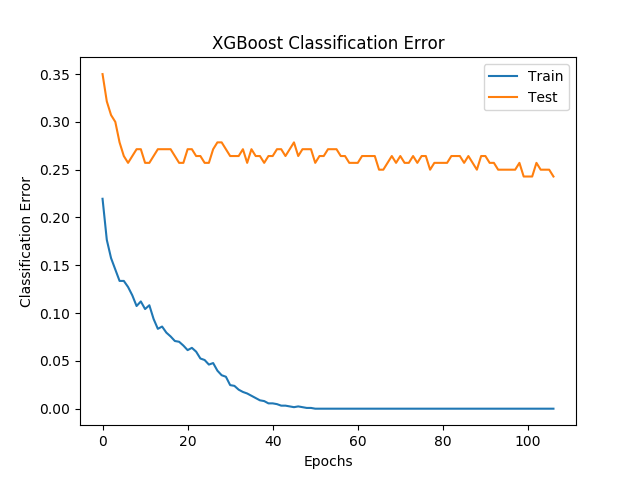
\includegraphics[width=0.4\linewidth]{figures/plot_training_error.png}
      }
    	\hspace{0.02\linewidth}
      \subfloat{
          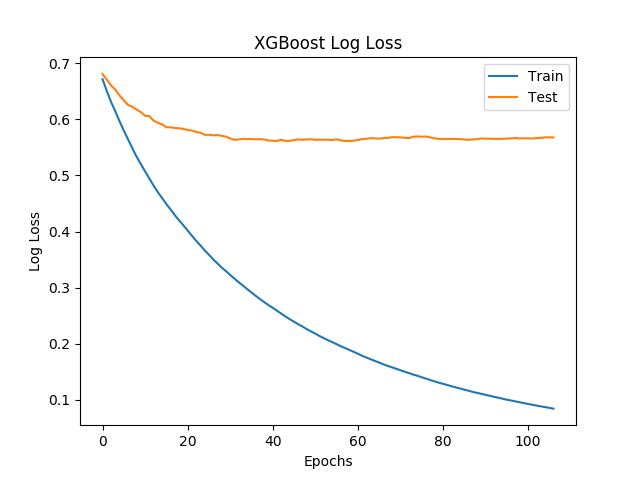
\includegraphics[width=0.4\linewidth]{figures/plot_training_logloss.png}
      }
      \hspace{0mm}
            \subfloat{
         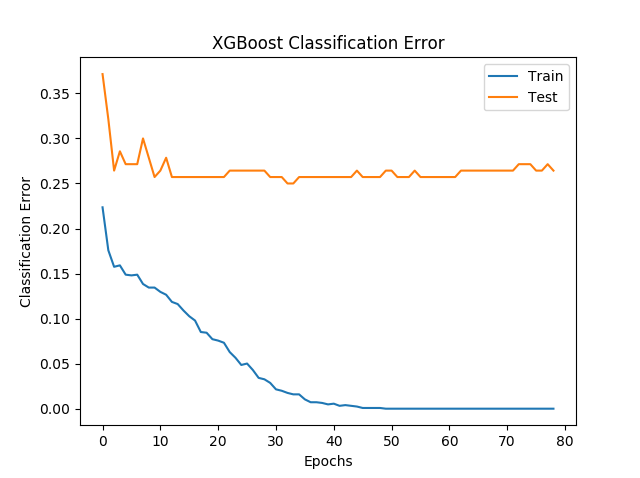
\includegraphics[width=0.4\linewidth]{figures/plot_training_error_random.png}
      }
    	\hspace{0.02\linewidth}
      \subfloat{
          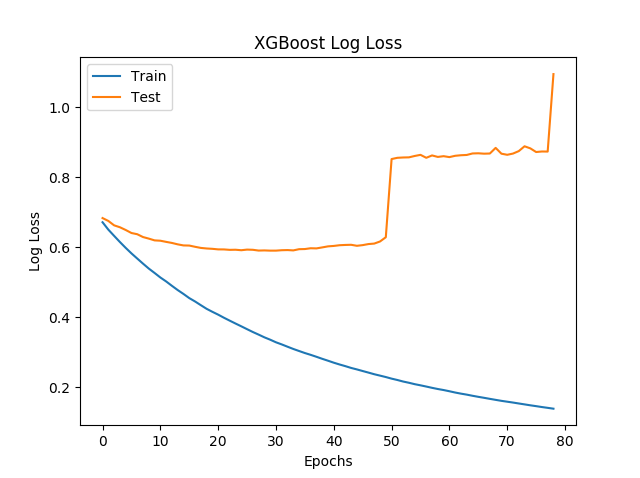
\includegraphics[width=0.4\linewidth]{figures/plot_training_logloss_random.png}
      }
      \caption{Classification and logloss of the training and testing set. The figures on the top are the baseline ResNet50 classifier. The figures on the bottom are from the random classifier. Classification figures on the left are thresholded values $v$ where $v > .5$ indicates the patient develops cancer.}
      \label{fig:training}
\end{figure}

On the first stage leaderboard, the submission of the feature transferred classifier placed 86th of 394 entries, with a logloss of .57616. On the second stage leaderboard, the classifier placed 265th of 394 entries, with a logloss of 0.66106. The distribution of the scores below a logloss of 1 are shown in \textit{Figure~\ref{fig:leaderboard}}.

%%% leaderboard
\begin{figure}[htb]
  \centering
  \begin{minipage}[c]{0.4\textwidth}
    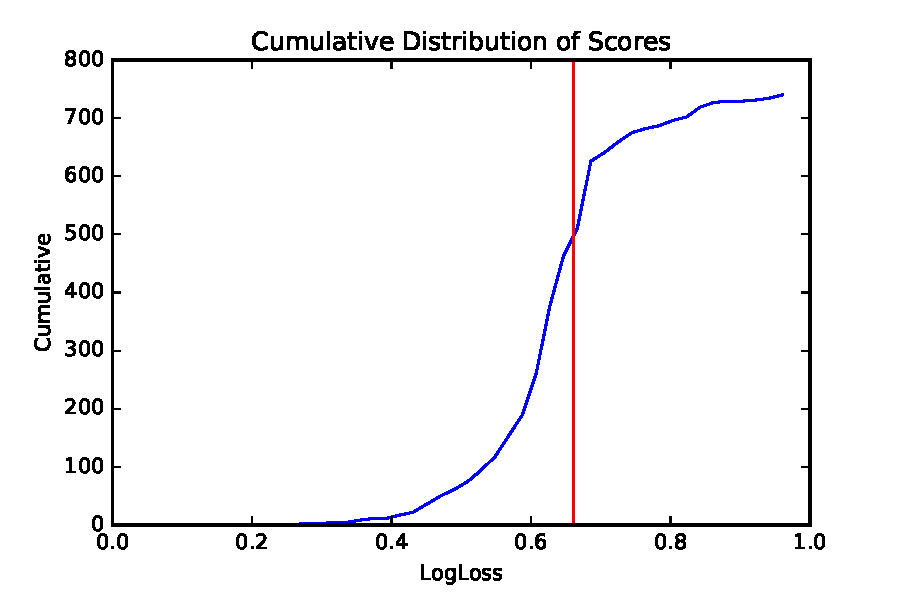
\includegraphics[width=\textwidth]{figures/plot_leaderboard.pdf}
  \end{minipage}
  \begin{minipage}[c]{0.4\textwidth}
    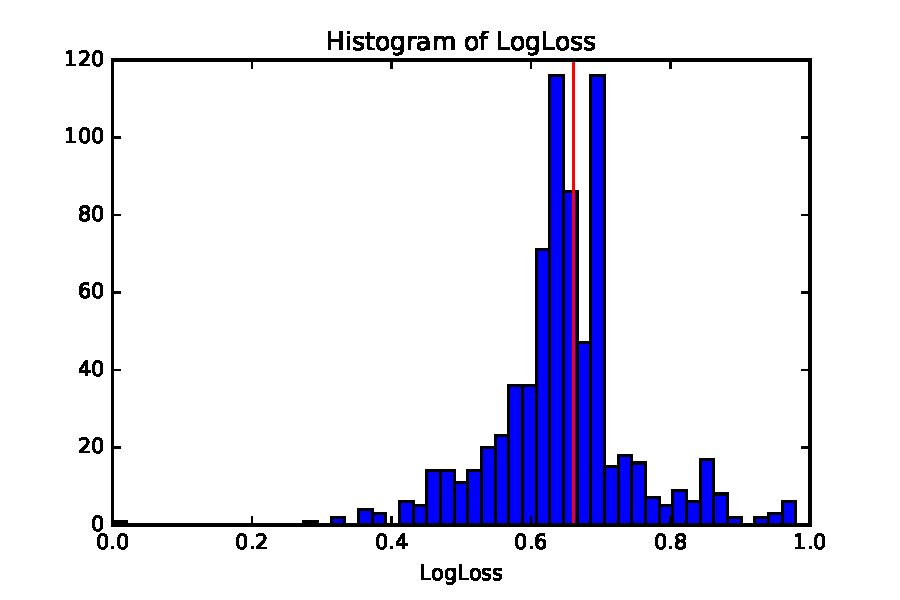
\includegraphics[width=\textwidth]{figures/leaderboard_histogram.pdf}
  \end{minipage}
  \caption{Cumulative distribution and histrogram of all entires on the logloss of stage2 within the competition. The red vertical lines indicate the baseline classifier. Only entries with less than 1 logloss are shown. The spike in distributions shows that many of the entries may have contained similar features and techniques. The 0 loss entry was a result of leaderboard hacking that does not qualify for the competition.}
  \label{fig:leaderboard}
\end{figure}

To evaluate the relative performance of the baseline versus random classifier, the receiver operating curve (ROC) can be used. An ROC curve is a measure of the performance of a binary classifier when the discrimination threshold is varied. The area under the curve (ROC-AUC), is a quantitative measurement of this value. An completely worst classifier would score an ROC-AUC of .5, with scores upper bounded by 1. The baseline ROC-AUC had a performance of .64 while random had .59 as show in \textit{Figure ~\ref{fig:roc}}.

%%% roc
\begin{figure}
    \centering
    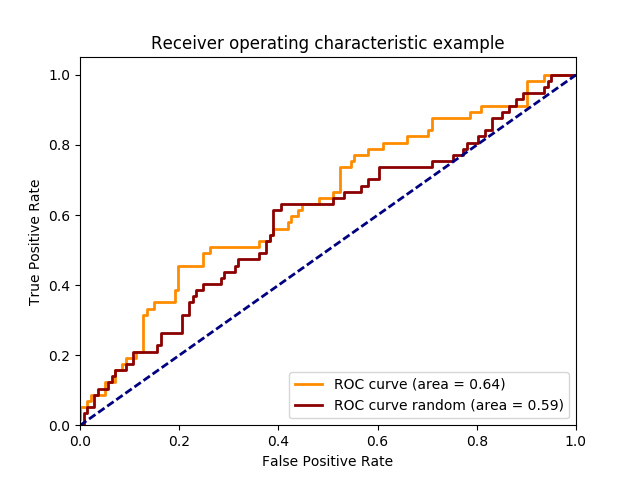
\includegraphics[width=0.8\linewidth]{figures/plot_roc_curves.png}
    \caption{The ROC curve for the random (red) and baseline (orange) classifier. The curve to beat (blue) shows both beat random performance.}
    \label{fig:roc}
\end{figure}

\section{Discussion \& Future Work}

As shown in the previous results, the baseline classifier implemented in this project outperformed the random classifier. The random classifier performed well within the training set error, meaning there was enough synchronized variation within the features to discern biases. When the random classifier was generalized to the test set, the performance degraded quickly over training epochs. This performance degradation was likely due to overfitting the training set, where the classifier was able to detect traits specific to the training set that did not generalize to the test set. However, the gradient boosting machine was able to detect features from the baseline ResNet50 semantic tagging network that generalized well within the testing set.

The way that this competition was structured allowed for the use of outside data. However, for the transfer learning purposes, no outside data was used that is in any similar to CT image data. The comparison of the random network to the feature transferred network showed the generalization of features being learned from neural networks. More work would be required to verify the results. The difference in ROC-AUCs (.05) may not seem significant enough to warrant conclusions. Other datasets might be required to verify the conclusions.

The significant differences in the stage1 versus stage2 leaderboards emphasizes the importance of model validation techniques. Specifically, the use of cross-validation allows for limiting the amount of information leakage between the training set and the test set. Many of the participants in this competition deployed techniques, such as probability clipping, to maximize their score on the stage1 leaderboard. However, if the distribution of risks within the stage1 leaderboard does not well represent the stage2 leaderboard, leaderboard information leakage can harm the models rather than help. This information leakage of the leaderboard was helpful for rough generalization estimates, but not complete in its information.

This paper showed showed the effectiveness of neural networks features to be transferred to new classification tasks. In this way, it was shown that feature transferring techniques can be useful for vastly different classification applications. However, this approach warrants many tasks that could improve the overall performance as outlined below.

\begin{itemize}
\item \textbf{Preprocesses} The images for this dataset were preprocessed in a specific way to utilize the pre-trained network architecture input shape and size. This approach could be improved by removing irrelevant parts of the image, such as segmenting to contain only the lungs in the scan.
\item \textbf{Backpropogation} The network features are not re-trained from their original task. This is the equivalent of teaching a person to fish, and then asking them to farm. The network and the error with the gradient boosting machine could be backpropogated after the initialization.
\item \textbf{Network Architecture} The network architecture used in these experiments were optimized for the 2D convolution operations on images with three color channels. However, for the purposes of CT Scans, the images are 3D with a single channel. If the network was altered to fit this data shape and size results could increase. A basic 3D CNN was trained on this data, but due to the sample size, it did nothing but fit and predict the majority class. Larger sample size would be required to fulfill this requirement.
\item \textbf{Summarization Techniques} A simple mean of the various slices was used to summarize the various sized scans. Other techniques, such as median and variance were used, but nothing performed better. This is complicating, because a single slice could contain the prediction for the entire image. Thus, it is most likely that other techniques could be used for summarization, such as max that could better standardize the data.
\end{itemize}

\section{Conclusion}

The objective of the Science Bowl was to increase the true positive rate of early stage cancer diagnosis from a CT scan. The creators of the competition were interested in the ability of artificial intelligence to synergize with human expert knowledge. The results of the competition allowed for a lot of the automation of this procedure. The winners of the competition used a segment then classify approach, similar to that of what a radiologist would do. They used external data, labeled by humans with nodules and malignancy. Then, the number of nodules detected from a given scan were reduced through a false positive reduction network. Finally, each nodule was classified individually for their malignancy and then combined for the best score. This sort of approach can help radiologists identify nodules that they might have missed in their looking throughout the data. If a malignant nodule is missed by the radiologist within the segmentation stages, the diagonsis of the entire scan becomes incorrect. This CAD design would help radiologists with identifying and narrowing the set of potential malignant nodules, as well as classifying the patient.

The approach outlined in this paper utilized the weights of a pre-trained network from an entirely different classification task. The results of the experiment showed that this baseline classifier, when compared to a classifier with random weights, outperformed a majority class classifier as well as the random classifier. This finding shows the phenomena of networks generalizable, and how pre-trained networks can be used for initialization of network weights rather than random weights to help with convergence.

%\onecolumn
%\section{Appendix A}

\bibliography{myrefs}
\bibliographystyle{IEEEtran}

\end{document}

